\subsection{Benchmarking}
The process of analyzing the sound files in the field of soundscape ecology is quite painful as it stands. Currently, our sponsor uses wav format sound files of size 1.29GB, each a recording of sixty minutes long. Some datasets used include over one hundred sound files, which amounts to over 100GB of sound files to process. It is important to know the length of time needed to process these files locally based on the end user\textquotesingle s hardware. The following are the results of NDSI index analysis on a single sound file of size 1.29GB, and the respective hardware involved. In addition, results for file splicing are included as results of this research. As a side note, it seems important to add that in order to run analysis on sound files in R, each wav file must be converted to a Wave object in R to be used in the index processes. This alone has proven to be a lengthy process on lower end systems.\\

\subsubsection{Large File Analysis}

\noindent\textbf{System 1: Intel i5 6500 4 Cores @ 3.2GHz / 16GB RAM}\\
The analysis took 686.64 seconds to process a single 1.29GB wav sound file. That comes out to 1.29GB in eleven minutes and forty four seconds. For a data set comprised of one hundred 1.29GB sound files, that would estimate to around nineteen hours for 129GB of sound files.\\

\noindent\textbf{System 2: Intel i7 7500U 2 Cores @ 2.7GHz / 16GB RAM}\\
The analysis took 1045.95 seconds to process a single 1.29GB wav sound file. That comes out to 1.29GB in seventeen minutes and twenty five seconds. For a data set comprised of one hundred 1.29GB sound files, that would estimate to around twenty nine hours for 129GB of sound files.\\

\noindent\textbf{System 3: Intel i5 5200U 2 Cores @ 2.2GHz / 8GB RAM}\\
The process of converting this single wav file to a Wave object in R actually managed to freeze this system for around 30 minutes, before any analysis even began. Then after 315.4 seconds, a little over five minutes, the processing stopped with an error reading "cannot allocate vector of size 1.3GB." This was an unexpected result, raising questions as to possible user minimum required hardware specs. Thus, with this hardware, processing is not even feasible.\\

\noindent\textbf{System 4: Intel i7 6500U 4 Cores @ 3.1GHz / 24GB RAM}\\
The analysis took 585.19 seconds to process a single 1.29GB wav sound file. That comes out to 1.29GB in nine minutes and forty five seconds. For a data set comprised of one hundred 1.29GB sound files, that would estimate to around sixteen hours for 129GB of sound files.\\

\noindent\textbf{System 5: Intel i7 7700HQ 4 Cores @ 2.8GHz / 16GB RAM}\\
The analysis took 690 seconds to process a single 1.29GB wav sound file. That comes out to 1.29GB in eleven minutes and thirty seconds. For a data set comprised of one hundred 1.29GB sound files, that would estimate to around nineteen hours for 129GB of sound files.\\

\noindent\textbf{System 6: Intel i5 5200U 4 Cores @ 2.7GHz / 8GB RAM}\\
This system also could not manage to process the sound file due to memory issues. Again, processing with these specs is infeasible.\\

\noindent\textbf{Solutions}\\
A solution to the issue of memory problems and processing time is the splitting of sound files into smaller pieces. Currently, each file is sixty minutes long. The sample file used was cut into six, ten minute parts, still retaining the wav file type. The NDSI processing time improved a bit on System 1, with each file taking  about 102.41 seconds, coming to about ten minutes. Further, when attempting to run the ACI index on System 1 \textit{without} splitting the file, it could not be done due to memory issues, even at 16GB of RAM. However when splitting the file, not only could the processing occur succesfully, it did so in 29.33 seconds, almost three minutes for all six files. This is much more reasonable and successful all around, and will be implemented into the service. Luckily the \codesnip{soundecology} package includes parameters for splitting up large files into smaller sections for analysis, which solves some of these issues.\\

\noindent\textbf{Conclusions}\\
From the benchmarks above, it seems that some minimum user requirements could be placed. Both systems that failed to process had no more than 8GB of RAM, drawing the conclusion that more than 8GB is required, at least for NDSI. For ACI though, even 16GB was not enough. As for processing speeds and processor core numbers, the following analysis can be made.\par
The only outlier that can be seen is System 5. This system had the same number of cores and RAM storage as the other systems, but with a much lower processing time compared to System 2, and a similar processing time compared to System 1. For System 2, this system compared to System 5 has the only difference of core numbers. What is interesting is that System 1 has a .4GHz clock speed advantage over System 5, yet a very similar processing time. The reasoning for this similarity is currently unknown.\par
The lowest recorded processing time was from System 4. System 4 had both the highest RAM storage and the second highest processing speed, only behind by .1GHz to System 1.\par
It is safe to conclude that RAM storage plays an important part in analysis here when comparing System 2 and System 6. Both have a clock speed of 2.7GHz, however System 6 only has 8GB of RAM. Along with System 2, these systems had the lowest amount of RAM out of those tested, and it can be concluded that 8GB of RAM is not enough for the processing of large sound files. Research on performance increases when splitting the files can be found in the next section.\par

\subsubsection{File Splitting Analysis}
The purpose of this section is to run some analysis on the performance benefits of splitting up sound files into smaller portions. As mentioned above, sixty minute, 1.29GB sound files are too large to compute even on high end systems. Thus, some research must be done to find the most efficient format for processing. The following results are all ACI index run using System 1, and on the same sound file from the Benchmarking section above. Keep in mind that the ACI index could not be processed on System 1 using the sixty minute file due to memory constraints.\\

\noindent\textbf{One Minute Splits}\\
The analysis took 2.45 seconds to process a the first minutes of the wav sound file. The analysis took 2.48 seconds to process the next minute of the wav sound file. Thus, it is assumed that these splits all come out to around two and a half seconds of processing time per minute. To do the whole sixty minutes, it would take about two minutes and thirty seconds using one minute splits.\\

\noindent\textbf{Five Minute Splits}\\
The analysis took 14.15 seconds to process a the first five minutes of the wav sound file. The analysis took 14.06 seconds to process the next five minutes of the wav sound file. Thus, it is assumed that these splits all come out to around fourteen seconds of processing time per five minutes. To do the whole sixty minutes, it would take about two minutes and fourty eight seconds using five minute splits.\\

\noindent\textbf{Ten Minute Splits}\\
The analysis took 30.09 seconds to process a the first ten minutes of the wav sound file. The analysis took 29.00 seconds to process the next ten minutes of the wav sound file. Thus, again it can be assumed that these splits all come out to around thirty seconds of processing time per ten minutes. To do the whole sixty minutes, it would take about three minutes using ten minute splits.\\

\noindent\textbf{Fifteen Minute Splits}\\
The analysis took 44.20 seconds to process a the first fifteen minutes of the wav sound file. The analysis took 43.51 seconds to process the next fifteen minutes of the wav sound file. Thus, it can be assumed that these splits all come out to around forty four seconds of processing time per fifteen minutes. To do the whole sixty minutes, it would take about two minutes and fifty four seconds using fifteen minute splits.\\

\noindent\textbf{Twenty Minute Splits}\\
The analysis took 59.46 seconds to process a the first twenty minutes of the wav sound file. The analysis took 58.54 seconds to process the next twenty minutes of the wav sound file. Thus, it can be assumed that these splits all come out to around fifty nine seconds of processing time per twenty minutes. To do the whole sixty minutes, it would take about two minutes and fifty seven seconds using twenty minute splits.\\

\noindent\textbf{Thirty Minute Splits}\\
The analysis took 134.63 seconds to process a the first thirty minutes of the wav sound file. The analysis took 117.55 seconds to process the last thirty minutes of the wav sound file. This is a range of about seventeen seconds, so best case scenario we are looking at just under two minutes for thirty seconds. To do the whole sixty minutes, it would take about three minutes and fifty five seconds using thirty minute splits. This is much higher than all the other splits, which comes as a surprise.\\

\noindent\textbf{Conclusions}\\
\begin{center}
	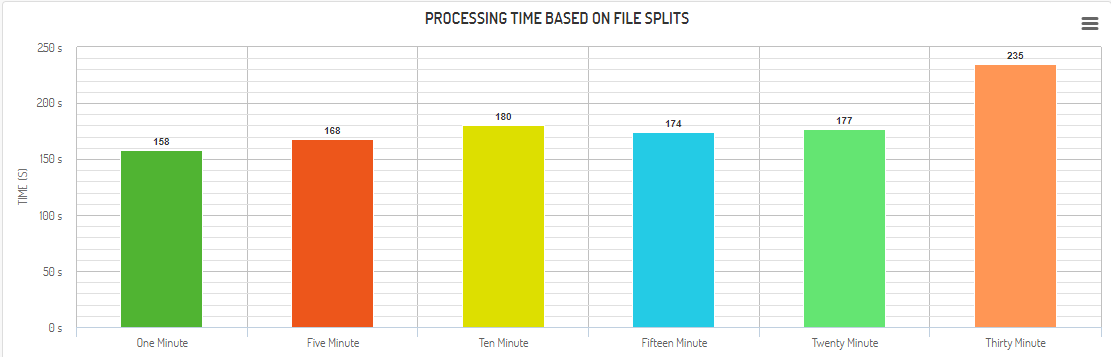
\includegraphics[width=\textwidth]{fileSplits}
\end{center}
Interestingly, all the different splits performed mostly the same \textit{except} for the thirty minute splits. Further, the ten minute splits ended up a tad bit higher than even the fifteen and twenty minute splits. The lowest recorded time was the one minute splits, and the highest being the thirty minute splits. Going forward, this research helps us make the decision on how to split the files up to maximize performance, especially on lower end systems. It seems that one to five minute splits will be the best choice.

\paragraph{Conclusions} \mbox{}\\[\paragraphheaderspace]
\begin{center}
	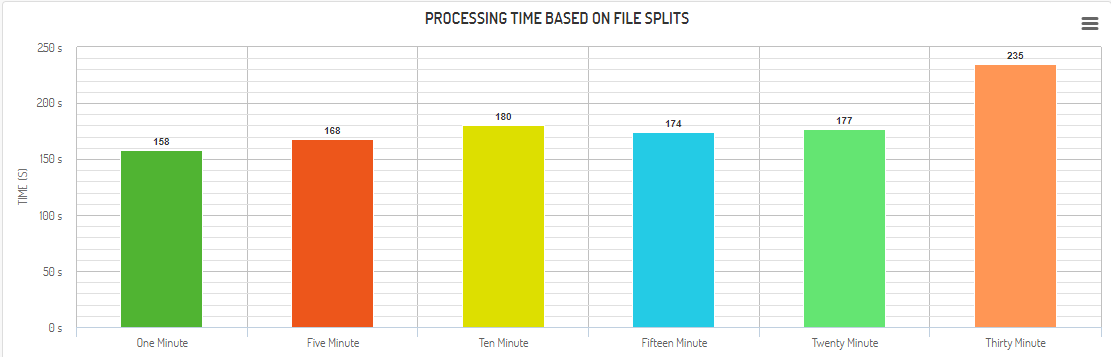
\includegraphics[width=\textwidth]{fileSplits}
\end{center}
Interestingly, all the different splits performed mostly the same \textit{except} for the thirty minute splits. Further, the ten minute splits ended up a tad bit higher than even the fifteen and twenty minute splits. The lowest recorded time was the one minute splits, and the highest being the thirty minute splits. Going forward, this research helps us make the decision on how to split the files up to maximize performance, especially on lower end systems. It seems that one to five minute splits will be the best choice.\par
Interestingly, all the different splits performed mostly the same \textit{except} for the thirty minute splits. Further, the ten minute splits ended up a tad bit higher than even the fifteen and twenty minute splits. The lowest recorded time was the one minute splits, and the highest being the thirty minute splits. Going forward, this research helps us make the decision on how to split the files up to maximize performance, especially on lower end systems. It seems that one to five minute splits will be the best choice.\par
It seems that some minimum user requirements could be placed. Both systems that failed to process had no more than 8GB of RAM, drawing the conclusion that more than 8GB is required, at least for NDSI. For ACI though, even 16GB was not enough. As for processing speeds and processor core numbers, the following analysis can be made.\par
The only outlier that can be seen is System 5. This system had the same number of cores and RAM storage as the other systems, but with a much lower processing time compared to System 2, and a similar processing time compared to System 1. For System 2, this system compared to System 5 has the only difference of core numbers. What is interesting is that System 1 has a .4GHz clock speed advantage over System 5, yet a very similar processing time. The reasoning for this similarity is currently unknown.\par
The lowest recorded processing time was from System 4. System 4 had both the highest RAM storage and the second highest processing speed, only behind by .1GHz to System 1.\par
It is safe to conclude that RAM storage plays an important part in analysis here when comparing System 2 and System 6. Both have a clock speed of 2.7GHz, however System 6 only has 8GB of RAM. Along with System 2, these systems had the lowest amount of RAM out of those tested, and it can be concluded that 8GB of RAM is not enough for the processing of large sound files. Research on performance increases when splitting the files can be found in the next section.\par
Through further analysis and research, it was discovered that file splitting actually has some negative effects on the validity of the outputs. When file splitting, the output of indices such as NDSI and ACI do not align with the output of the same file without splitting. When it comes to research taking place by the user, this is unacceptable and will invalidate any research done. Thus, it was decided to not include file splitting despite the performance enhancements on some systems, for the sake of data validity. In the future, it may be possible to negate the effects of file splitting, or to add the option for it with a disclaimer.

